%
% LaTeX report template 
%

% This is a comment: in LaTeX everything that in a line comes
% after a "%" symbol is treated as comment

\documentclass[11pt, a4paper]{article}
\usepackage{graphicx}
\usepackage{amsmath}
\usepackage{listings}
\usepackage[font=scriptsize]{caption}
\usepackage{caption}
\title{Assignment No 4} % Title

\author{Prasanna Bartakke EE19B106} % Author name

\date{\today} % Date for the report
\begin{document}		
		
\maketitle % Insert the title, author and date
\section{Visualising the functions}
%Create new section;it is autonumbered
The functions $e^x$ and $cos(cos(x))$ are plotted over the interval $[-2\pi, 4\pi)$ using 500 points which are sampled uniformly over this interval.

\begin{figure}
\centering
\begin{minipage}{.5\textwidth}
  \centering
  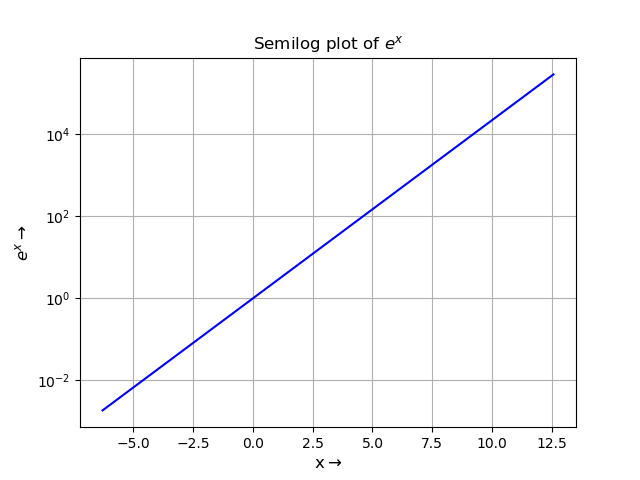
\includegraphics[width=\linewidth]{fig1.png}
  \captionof{figure}{Semilog plot of $e^x$}
  \label{fig:test1}
\end{minipage}%
\begin{minipage}{.5\textwidth}
  \centering
  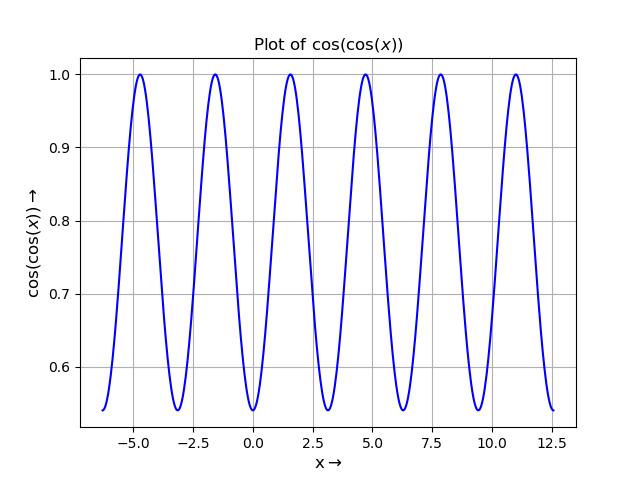
\includegraphics[width=\linewidth]{fig2.png}
  \captionof{figure}{Plot of $cos(cos(x))$}
  \label{fig:test2}
\end{minipage}
\end{figure}

The function $e^x$ is increasing and non-periodic. The function $cos(cos(x))$ is periodic with period $\pi$. 
The Fourier series will give us the expression for the function in terms of $2\pi$ periodic signals. As the function $e^x$ is aperiodic, its Fourier series is calculated by taking the function in he interval $[0, 2\pi)$ and repeating it to get a $2\pi$ periodic function. As the function $e^x$ increases rapidly, it can be represented by only high frequency sinusoids. Thus Fourier series would yield a reasonable approximation for large number of coefficients.
$cos(cos(x))$ has a period of $\pi$, so the Fourier series yields almost exact approximation for the function.

\section{Fourier series coefficients}

The Fourier series coefficients are calculated using the integrate.quad function in the scipy library. The following code snippet evaluates the first n coefficients of the Fourier transform of a given function. Thus the first 51 coefficients of the two functions are obtained and are plotted below.

 
 
\begin{figure}
\centering
\begin{minipage}{.5\textwidth}
  \centering
  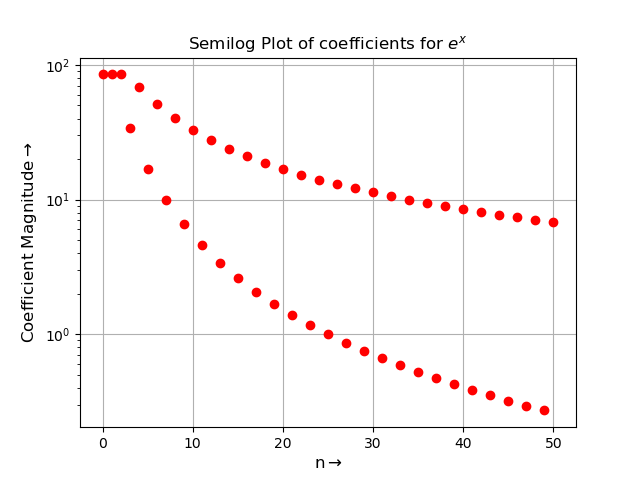
\includegraphics[width=0.9\linewidth]{fig3.png}
  \captionof{figure}{Semilog plot of coefficients of $e^x$}
  \label{fig:test1}
\end{minipage}%
\begin{minipage}{.5\textwidth}
  \centering
  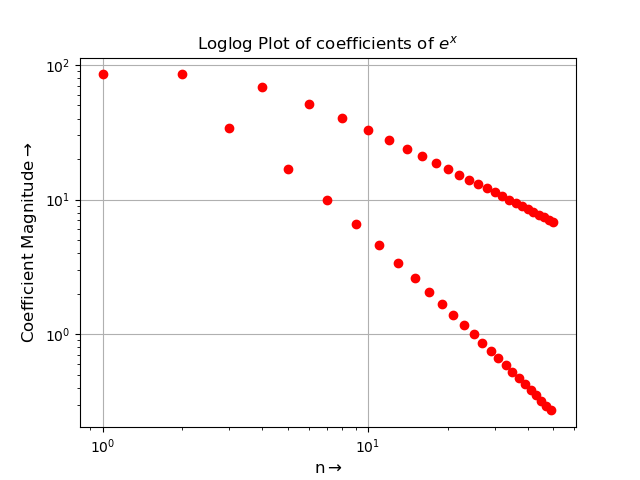
\includegraphics[width=\linewidth]{fig4.png}
  \captionof{figure}{Log plot of coefficients of $e^x$}
  \label{fig:test2}
\end{minipage}
\end{figure}

\begin{figure}
\centering
\begin{minipage}{.5\textwidth}
  \centering
  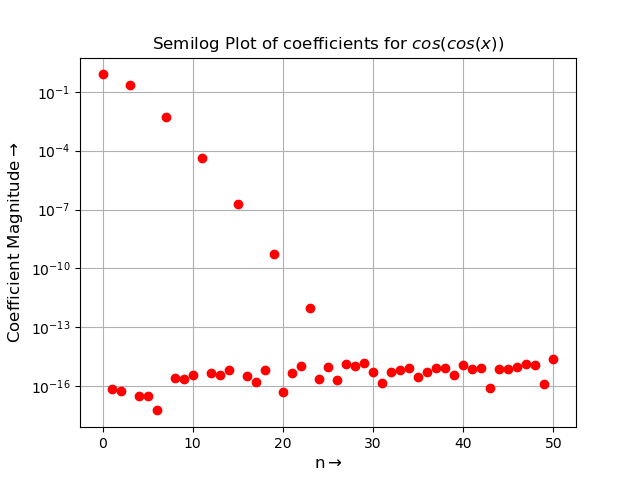
\includegraphics[width=0.9\linewidth]{fig5.png}
  \captionof{figure}{Semilog plot of coefficients of $cos(cos(x))$}
  \label{fig:test1}
\end{minipage}%
\begin{minipage}{.5\textwidth}
  \centering
  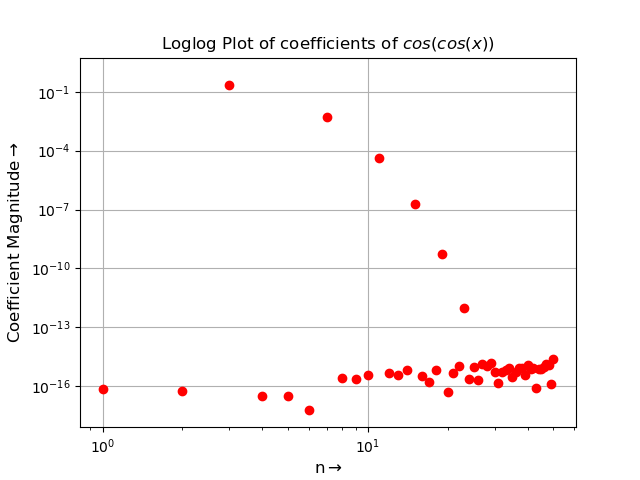
\includegraphics[width=\linewidth]{fig6.png}
  \captionof{figure}{Log plot of coefficients of $cos(cos(x))$}
  \label{fig:test2}
\end{minipage}
\end{figure}

 \begin{verbatim}	
def fourier_transform(n, function):
    coeff = np.zeros(n)
    def u(x, k, f):
        return f(x)*np.cos(k*x)/np.pi
    def v(x,k,f):
        return f(x)*np.sin(k*x)/np.pi

    coeff[0] = integrate.quad(function,0,2*np.pi)[0]/(2*np.pi)
    for i in range(1,n):
        if i%2:
            coeff[i] = integrate.quad(u,0,2*np.pi,args=((i//2) +1,function))[0]
        else:
            coeff[i] = integrate.quad(v,0,2*np.pi,args=(i//2,function))[0]
    return coeff 
\end{verbatim}
 
 The $b_n$ coefficients of $cos(cos(x))$ should be zero as $cos(cos(x))$ is an even function. However, the values obtained are non-zero due to the limitation in numerical accuracy upto which $\pi$ can be stored in the memory.
 As the first function is exponentially increasing, it contains a wide range of frequencies in its Fourier transform. On the other hand, $cos(cos(x))$ has frequency $\dfrac{1}{\pi}$, thus making the contribution by higher frequency sinusoids less, which results in the quick decay of coefficients with n.
 
 \[ \int_{0}^{2\pi} e^x cos(kx) \,dx  = \dfrac{e^{2\pi} - 1}{k^2 + 1}\] and
  \[ \int_{0}^{2\pi} e^x sin(kx) \,dx  = \dfrac{-ke^{2\pi} + k}{k^2 + 1}\]
 As we can see from the above intergrals, the loglog plot of $e^x$ is nearly linear.
Similarly, the coefficients of $cos(cos(x))$ are approximately exponential with n, thus the semilog plot is linear.

 
 
 \section{Least Squares Approach}
 The Fourier coefficients can be approximated by solving the matrix equation $Ac = b$, where 
 
 \begin{equation}
 A = 
 \begin{bmatrix}
 1 & cos(x_1) & sin(x_1) & .... & cos(25x_1) & sin(25x_1)\\
 1 & cos(x_2) & sin(x_2) & .... & cos(25x_2) & sin(25x_2)\\
 ... & ... & ... & .... & ... & ...\\
 1 & cos(x_{400}) & sin(x_{400}) & .... & cos(25x_{400}) & sin(25x_{400})
\end{bmatrix}
b = 
\begin{bmatrix}
 f(x_1)\\
 f(x_2)\\
 ...\\
 f(x_{400})\\
\end{bmatrix}
 \end{equation}
The plots obtained are given below.
\begin{figure}
\centering
\begin{minipage}{.5\textwidth}
  \centering
  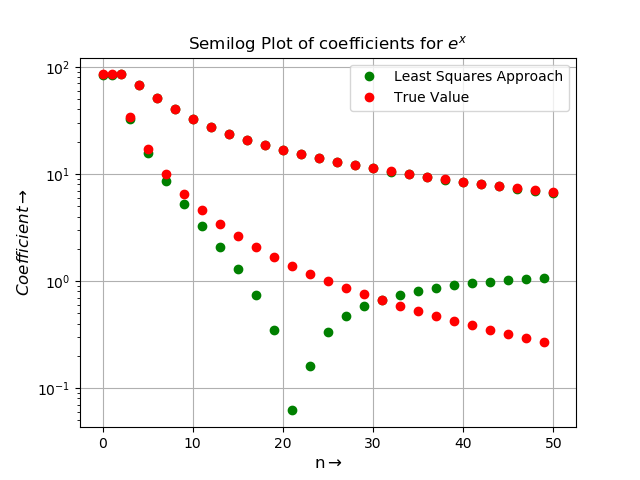
\includegraphics[width=\linewidth]{fig7.png}
  \captionof{figure}{Semilog plot of coefficients of $e^x$}
  \label{fig:test1}
\end{minipage}%
\begin{minipage}{.5\textwidth}
  \centering
  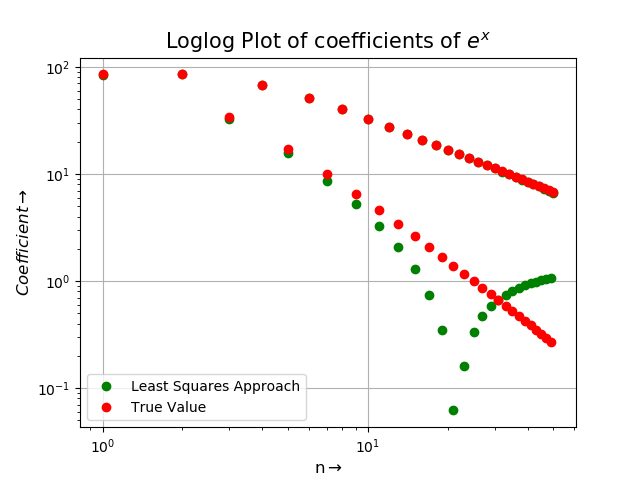
\includegraphics[width=\linewidth]{fig8.png}
  \captionof{figure}{Log plot of coefficients of $e^x$}
  \label{fig:test2}
\end{minipage}
\end{figure}

\begin{figure}
\centering
\begin{minipage}{.5\textwidth}
  \centering
  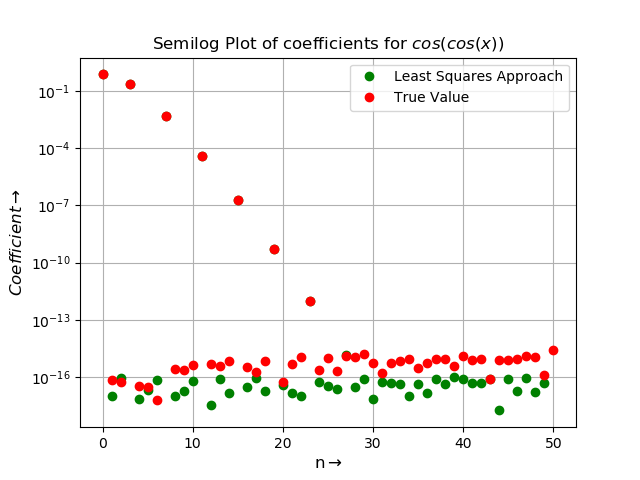
\includegraphics[width=\linewidth]{fig9.png}
  \captionof{figure}{Semilog plot of coefficients of $cos(cos(x))$}
  \label{fig:test1}
\end{minipage}%
\begin{minipage}{.5\textwidth}
  \centering
  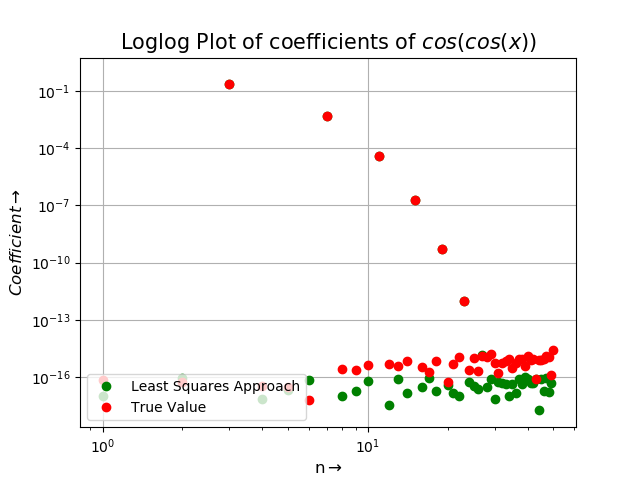
\includegraphics[width=\linewidth]{fig10.png}
  \captionof{figure}{Log plot of coefficients of $cos(cos(x))$}
  \label{fig:test2}
\end{minipage}
\end{figure}

\section{Function Approximation}
The product, $P = Ac$ gives an estimate of the function values at $\{x_1, x_2, ..., x_{400}\}$. These estimates along with the actual functions are plotted below.
\begin{figure}[!tbh]
   	\centering
   	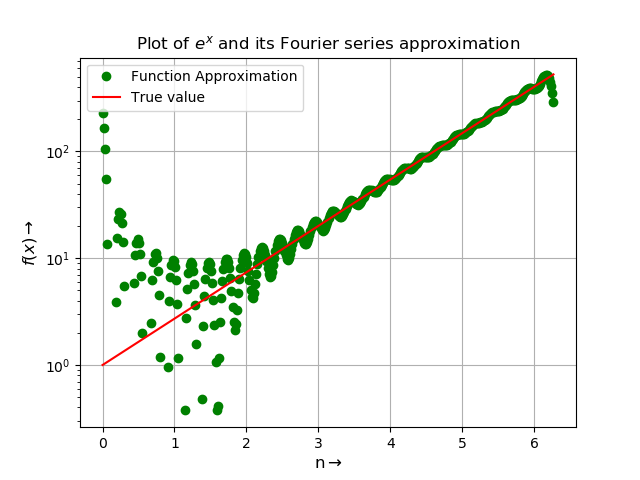
\includegraphics[scale=0.5]{fig11.png}  % Mention the image name within the curly braces. Image should be in the same folder as the tex file. 
   	\caption{Plot of $e^x$ and its Fourier series approximation.}
   	\label{fig:sample}
   \end{figure} 

\begin{figure}[!tbh]
   	\centering
   	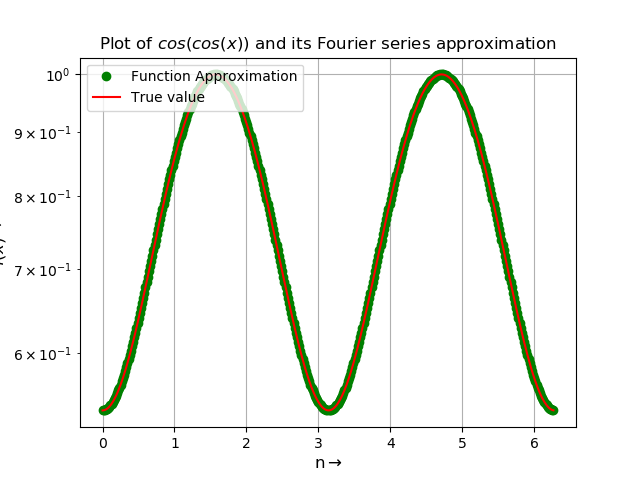
\includegraphics[scale=0.5]{fig12.png}  % Mention the image name within the curly braces. Image should be in the same folder as the tex file. 
   	\caption{Plot of $cos(cos(x))$ and its Fourier series approximation.}
   	\label{fig:sample}
   \end{figure} 
   
 There is a significant deviation in the case of $e^x$ as we need to consider higher frequency sinusoids. In case of $cos(cos(x))$ the estimate is exactly equal to the original function as the period is small($\pi$).
 
 \section{Conclusion}
 After finding the Fourier series coefficients of the function $e^x$ and $cos(cos(x))$ using two different methods, integration and estimation with least squares mathod, we find that the least squares method is computationally inexpensive than integration. Also we verified that odd sinusoidal components of $cos(cos(x))$ are zero. It was found out that least squares estimate deviates more for $e^x$ than $cos(cos(x))$, due to the aperiodic nature of $e^x$.
\end{document}



 